\documentclass{article}

\usepackage{cancel}
\usepackage{algorithm} %pseudo-code
\usepackage{algpseudocode}
\usepackage[columnsep=1cm, top=1cm, bottom=1.5cm, left=1cm, right=1cm]{geometry}
\usepackage{amsmath,amsthm,amssymb}
\usepackage{graphicx}
\usepackage{float}
\usepackage{amsmath, amssymb, amscd}
\usepackage{alltt}
\usepackage{textcomp}
\usepackage{gensymb}
\usepackage{multicol}
\usepackage{tabularx}
\usepackage{units}
%\usepackage{mathpple}
%\usepackage{mathpazo}
\usepackage{fouriernc}
%\usepackage{euler}
\usepackage[mathscr]{euscript}

\newcommand{\N}{\mathbb{N}}
\newcommand{\Z}{\mathbb{Z}}
\newcommand{\R}{\mathbb{R}}
\newcommand{\bigo}{\mathcal{O}}
\newcommand{\G}{\mathcal{G}}
\newcommand{\V}{\mathcal{V}}
\newcommand{\E}{\mathcal{E}}
\newcommand{\K}{\mathcal{K}}
\newcommand{\T}{^\intercal}

\def\changemargin#1#2{\list{}{\rightmargin#2\leftmargin#1}\item[]}
\let\endchangemargin=\endlist 

\newcommand{\sups}[1]{\ensuremath{^{\textrm{#1}}}}
\newcommand{\subs}[1]{\ensuremath{_{\textrm{#1}}}}

\newcommand{\specialcell}[2][c]
{
  \begin{tabular}[#1]{@{}c@{}}#2\end{tabular}
}

\makeatletter
\newsavebox{\mybox}\newsavebox{\mysim}
\newcommand{\distras}[1]
{
  \savebox{\mybox}{\hbox{\kern3pt$\scriptstyle#1$\kern3pt}}%
  \savebox{\mysim}{\hbox{$\sim$}}%
  \mathbin{\overset{#1}{\kern\z@\resizebox{\wd\mybox}{\ht\mysim}{$\sim$}}}%
}
\makeatother

% aligned matrix negative signs:
\makeatletter
\renewcommand*\env@matrix[1][c]{\hskip -\arraycolsep
  \let\@ifnextchar\new@ifnextchar
  \array{*\c@MaxMatrixCols #1}}
\makeatother

%===============================================================================
% code highlighting :
\usepackage{listings}

% define custom colors :
\usepackage{color}
\definecolor{bg}{rgb}{0.96,0.96,0.85}
\definecolor{deepblue}{rgb}{0,0,0.5}
\definecolor{deepred}{rgb}{0.6,0,0}
\definecolor{deepgreen}{rgb}{0,0.5,0}

\usepackage{xcolor}
\renewcommand{\lstlistlistingname}{Code Listings}
\renewcommand{\lstlistingname}{Code Listing}
\definecolor{gray}{gray}{0.5}
\colorlet{commentcolour}{green!50!black}

\colorlet{stringcolour}{red!60!black}
\colorlet{keywordcolour}{magenta!90!black}
\colorlet{exceptioncolour}{yellow!50!red}
\colorlet{commandcolour}{blue!60!black}
\colorlet{numpycolour}{blue!60!green}
\colorlet{literatecolour}{magenta!90!black}
\colorlet{promptcolour}{green!50!black}
\colorlet{specmethodcolour}{violet}
\colorlet{indendifiercolour}{green!70!white}

\newcommand{\framemargin}{5ex}

\newcommand{\literatecolour}{\textcolor{literatecolour}}

\newcommand\Small{\fontsize{1.00}{5.0}\selectfont}

\newcommand\pythonstyle{\lstset{
%keepspaces=true,
language=python,
showtabs=true,
tab=,
tabsize=2,
basicstyle=\ttfamily\Small,%\setstretch{.5},
stringstyle=\color{stringcolour},
showstringspaces=false,
alsoletter={1234567890},
otherkeywords={\ , \}, \{, \%, \&, \|},
keywordstyle=\color{keywordcolour}\bfseries,
emph={and,break,class,continue,def,yield,del,elif ,else,%
except,exec,finally,for,from,global,if,import,in,%
lambda,not,or,pass,print,raise,return,try,while,assert},
emphstyle=\color{blue}\bfseries,
emph={[2]True, False, None},
emphstyle=[2]\color{keywordcolour},
emph={[3]object,type,isinstance,copy,deepcopy,zip,enumerate,reversed,list,len,dict,tuple,xrange,append,execfile,real,imag,reduce,str,repr},
emphstyle=[3]\color{commandcolour},
emph={Exception,NameError,IndexError,SyntaxError,TypeError,ValueError,OverflowError,ZeroDivisionError},
emphstyle=\color{exceptioncolour}\bfseries,
%upquote=true,
morestring=[s]{"""}{"""},
morestring=[s]{'''}{'''},
commentstyle=\color{commentcolour}\slshape,
%emph={[4]1, 2, 3, 4, 5, 6, 7, 8, 9, 0},
emph={[4]ode, fsolve, sqrt, exp, sin, cos, arccos, pi,  array, norm, solve, dot, arange, , isscalar, max, sum, flatten, shape, reshape, find, any, all, abs, linspace, legend, quad, polyval,polyfit, hstack, concatenate,vstack,column_stack,empty,zeros,ones,rand,vander,grid,pcolor,eig,eigs,eigvals,svd,qr,tan,det,logspace,roll,min,mean,cumsum,cumprod,diff,vectorize,lstsq,cla,eye,xlabel,ylabel,squeeze,plot,median,std,hist},
emphstyle=[4]\color{numpycolour},
emph={[5]__init__,__add__,__mul__,__div__,__sub__,__call__,__getitem__,__setitem__,__eq__,__ne__,__nonzero__,__rmul__,__radd__,__repr__,__str__,__get__,__truediv__,__pow__,__name__,__future__,__all__},
emphstyle=[5]\color{specmethodcolour},
emph={[6]assert,range,yield},
emphstyle=[6]\color{keywordcolour}\bfseries,
% emph={[7]self},
% emphstyle=[7]\bfseries,
literate=*%
{:}{{\literatecolour:}}{1}%
{=}{{\literatecolour=}}{1}%
{-}{{\literatecolour-}}{1}%
{+}{{\literatecolour+}}{1}%
{*}{{\literatecolour*}}{1}%
{/}{{\literatecolour/}}{1}%
{!}{{\literatecolour!}}{1}%
%{(}{{\literatecolour(}}{1}%
%{)}{{\literatecolour)}}{1}%
{[}{{\literatecolour[}}{1}%
{]}{{\literatecolour]}}{1}%
{<}{{\literatecolour<}}{1}%
{>}{{\literatecolour>}}{1}%
{>>>}{{\textcolor{promptcolour}{>>>}}}{1}%
,%
breaklines=true,
breakatwhitespace= true,
%xleftmargin=\framemargin,
%xrightmargin=\framemargin,
aboveskip=1ex,
frame=trbl,
%frameround=tttt,
rulecolor=\color{black!40},
%framexleftmargin=\framemargin,
%framextopmargin=.1ex,
%framexbottommargin=.1ex,
%framexrightmargin=\framemargin,
%framexleftmargin=1mm, framextopmargin=1mm, frame=shadowbox, rulesepcolor=\color{blue},#1
%frame=tb,
backgroundcolor=\color{yellow!10}
}}

\newcommand\Rstyle{\lstset{
%keepspaces=true,
language=R,
showtabs=true,
tab=,
tabsize=2,
basicstyle=\ttfamily\Small,%\setstretch{.5},
stringstyle=\color{stringcolour},
showstringspaces=false,
alsoletter={1234567890},
otherkeywords={\ , \}, \{, \%, \&, \|},
keywordstyle=\color{keywordcolour}\bfseries,
emph={and,break,class,continue,def,yield,del,elif ,else,%
except,exec,finally,for,from,global,if,import,in,%
lambda,not,or,pass,print,raise,return,try,while,assert},
emphstyle=\color{blue}\bfseries,
emph={[2]True, False, None},
emphstyle=[2]\color{keywordcolour},
emph={[3]object,type,isinstance,copy,deepcopy,zip,enumerate,reversed,list,len,dict,tuple,xrange,append,execfile,real,imag,reduce,str,repr},
emphstyle=[3]\color{commandcolour},
emph={Exception,NameError,IndexError,SyntaxError,TypeError,ValueError,OverflowError,ZeroDivisionError},
emphstyle=\color{exceptioncolour}\bfseries,
%upquote=true,
morestring=[s]{"""}{"""},
morestring=[s]{'''}{'''},
commentstyle=\color{commentcolour}\slshape,
%emph={[4]1, 2, 3, 4, 5, 6, 7, 8, 9, 0},
emph={[4]ode, fsolve, sqrt, exp, sin, cos, arccos, pi,  array, norm, solve, dot, arange, , isscalar, max, sum, flatten, shape, reshape, find, any, all, abs, linspace, legend, quad, polyval,polyfit, hstack, concatenate,vstack,column_stack,empty,zeros,ones,rand,vander,grid,pcolor,eig,eigs,eigvals,svd,qr,tan,det,logspace,roll,min,mean,cumsum,cumprod,diff,vectorize,lstsq,cla,eye,xlabel,ylabel,squeeze,plot,median,std,hist},
emphstyle=[4]\color{numpycolour},
emph={[5]__init__,__add__,__mul__,__div__,__sub__,__call__,__getitem__,__setitem__,__eq__,__ne__,__nonzero__,__rmul__,__radd__,__repr__,__str__,__get__,__truediv__,__pow__,__name__,__future__,__all__},
emphstyle=[5]\color{specmethodcolour},
emph={[6]assert,range,yield},
emphstyle=[6]\color{keywordcolour}\bfseries,
% emph={[7]self},
% emphstyle=[7]\bfseries,
literate=*%
{:}{{\literatecolour:}}{1}%
{=}{{\literatecolour=}}{1}%
{-}{{\literatecolour-}}{1}%
{+}{{\literatecolour+}}{1}%
{*}{{\literatecolour*}}{1}%
{/}{{\literatecolour/}}{1}%
{!}{{\literatecolour!}}{1}%
%{(}{{\literatecolour(}}{1}%
%{)}{{\literatecolour)}}{1}%
{[}{{\literatecolour[}}{1}%
{]}{{\literatecolour]}}{1}%
{<}{{\literatecolour<}}{1}%
{>}{{\literatecolour>}}{1}%
{>>>}{{\textcolor{promptcolour}{>>>}}}{1}%
,%
breaklines=true,
breakatwhitespace= true,
%xleftmargin=\framemargin,
%xrightmargin=\framemargin,
aboveskip=1ex,
frame=trbl,
%frameround=tttt,
rulecolor=\color{black!40},
%framexleftmargin=\framemargin,
%framextopmargin=.1ex,
%framexbottommargin=.1ex,
%framexrightmargin=\framemargin,
%framexleftmargin=1mm, framextopmargin=1mm, frame=shadowbox, rulesepcolor=\color{blue},#1
%frame=tb,
backgroundcolor=\color{yellow!10}
}}

% Python environment
\lstnewenvironment{python}[1][]
{
  \pythonstyle
  \lstset{#1}
}
{}

% R environment
\lstnewenvironment{Rs}[1][]
{
  \Rstyle
  \lstset{#1}
}
{}

% Python for external files
\newcommand\pythonexternal[1]
{{
  \pythonstyle
  \lstinputlisting{#1}
}}

% R for external files
\newcommand\Rexternal[1]
{{
  \Rstyle
  \lstinputlisting{#1}
}}

% Python for inline
\newcommand\pythoninline[1]
{{
  \pythonstyle
  \lstinline!#1!
}}

% answer box :
\newcommand\answer[1]
{{
  \begin{center}
    \parbox[t]{5in}{#1}
  \end{center}
}}

% end code highlighting
%===============================================================================


% border matrix with brackets :
\usepackage{etoolbox}
\let\bbordermatrix\bordermatrix
\patchcmd{\bbordermatrix}{8.75}{4.75}{}{}
\patchcmd{\bbordermatrix}{\left(}{\left[}{}{}
\patchcmd{\bbordermatrix}{\right)}{\right]}{}{}


\begin{document}
\footnotesize

\title{Feature selection}
\author{Evan Cummings\\
CSCI 548 -- Douglas W.~Raiford -- Pattern Recognition}

\maketitle

\section{iris data}

\begin{figure}[H]
  %\centering
  \begin{minipage}[b]{0.45\linewidth}
    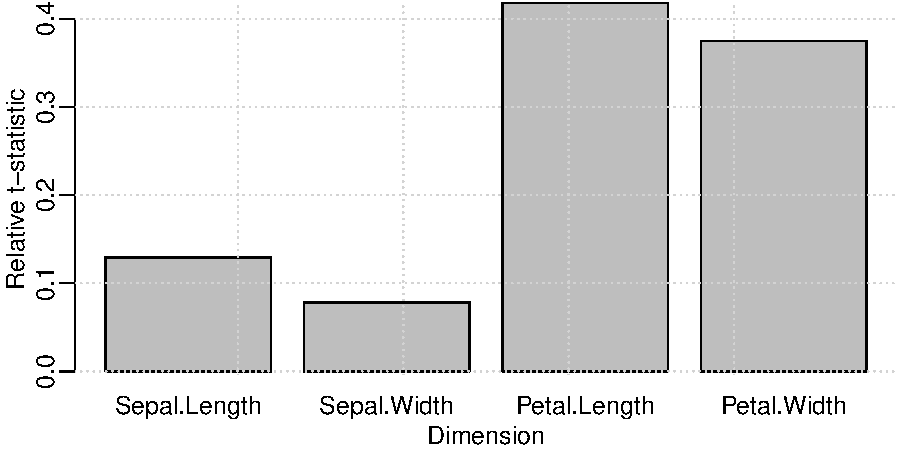
\includegraphics[width=\linewidth]{images/iris_ttest.pdf}
  \end{minipage}
  \hfill
  \quad
  \begin{minipage}[b]{0.45\linewidth}
    \centering
    \begin{tabular}[b]{c|lll}
      & \textbf{full} & \textbf{$t$-test} & \textbf{seq-fwrd} \\
      \hline
      rand.~acc.   & 97.4\% & 97.4\% & 97.4\% \\ 
      $n$-way acc. & 98\%   & 96\%   & 96\% \\
      dims         & all    & 3,4    & 1,3 \\
      $J_1$        & 6.50   & 15.2   & 7.41 \\
      $J_2$        & 41.7   & 22.4   & 24.6 \\
      $J_3$        & 31.8   & 19.4   & 22.9 \\
    \end{tabular}
    \vspace{5mm}
  \end{minipage}
  \hfill
  \vspace{5mm}
  \quad
  \begin{minipage}[t]{1.00\linewidth}
    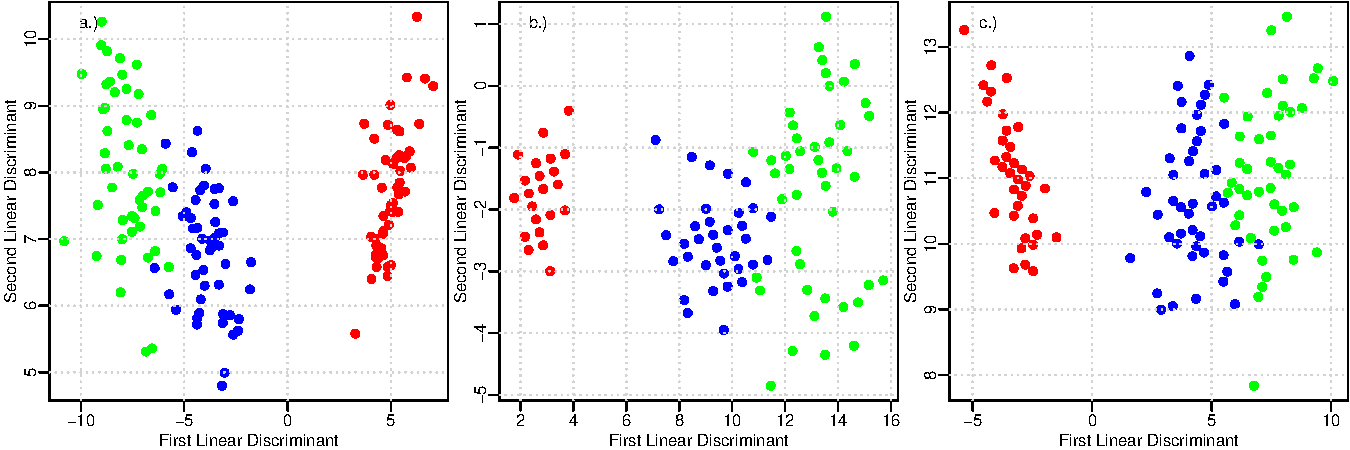
\includegraphics[width=\linewidth]{images/iris.pdf}
  \end{minipage}
  \caption{The \texttt{iris} data projected onto the first two linear discriminants using: a.) all the dimensions; b.) two best dimensions resulting from the relative-$t$-test (top left barplot); and c.), two best dimensions determined from the sequential-forward algorithm.  The random 75\% training data score, leave-one-out-cross-validation score, best dimension indicies, and $J$-scores are provided in the above right table for the full model, $t$-test-best-dimensions model, and sequential-forward-best-dimensions model.   Note that while both the $t$-test and sequential-forward models resulted in identical $n$-way-cross-validation scores, the $J_2$ and $J_3$ values associated with the sequential-forward model are slightly improved.}
\end{figure}

\section{fruit data}

\begin{figure}[H]
  %\centering
  \begin{minipage}[b]{0.45\linewidth}
    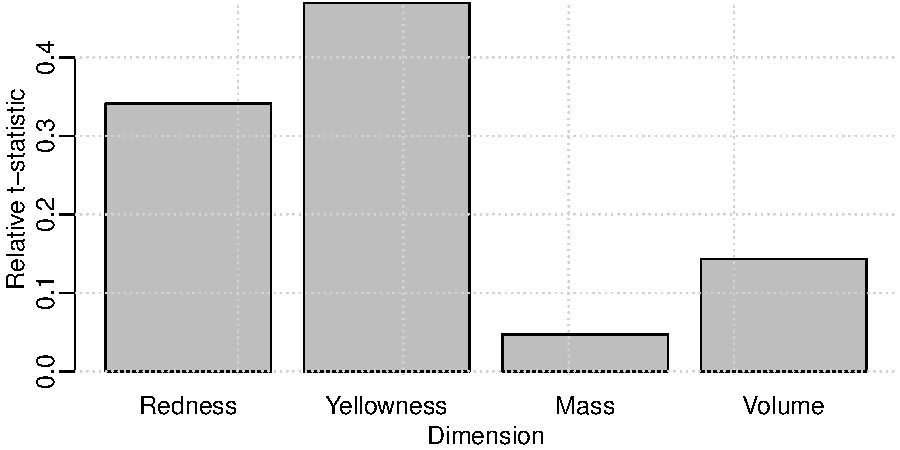
\includegraphics[width=\linewidth]{images/fruit_ttest.pdf}
  \end{minipage}
  \hfill
  \quad
  \begin{minipage}[b]{0.45\linewidth}
    \centering
    \begin{tabular}[b]{c|lll}
      & \textbf{full} & \textbf{$t$-test} & \textbf{seq-fwrd} \\
      \hline
      rand.~acc.   & 96.4\% & 95.6\%  & 95.6\% \\ 
      $n$-way acc. & 95.1\% & 94.1\%  & 94.1\% \\
      dims         & all    & 1,2     & 1,2 \\
      $J_1$        & 0.19   & 9.53    & 9.53 \\
      $J_2$        & 33.2   & 21.0    & 21.0 \\
      $J_3$        & 21.7   & 20.0    & 20.0 \\
    \end{tabular}
    \vspace{5mm}
  \end{minipage}
  \hfill
  \vspace{5mm}
  \quad
  \begin{minipage}[t]{1.00\linewidth}
    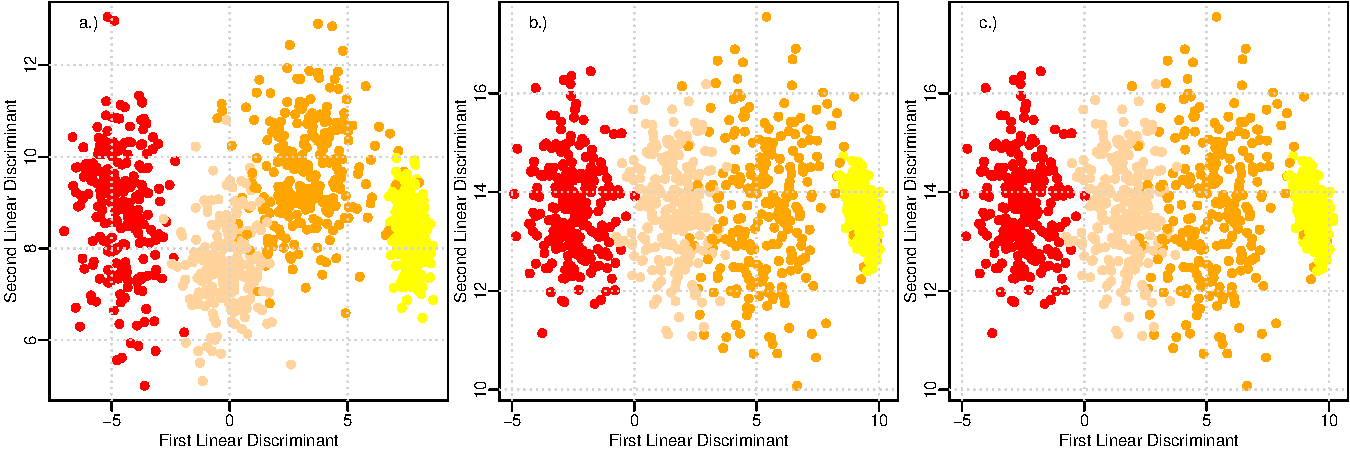
\includegraphics[width=\linewidth]{images/fruit.pdf}
  \end{minipage}
  \caption{The \texttt{fruit} data projected onto the first two linear discriminants using: a.) all the dimensions; b.) two best dimensions resulting from the relative-$t$-test (top left barplot); and c.), two best dimensions determined from the sequential-forward algorithm, in this case identical to those of the $t$-test.  The random 75\% training data score, leave-one-out-cross-validation score, best dimension indicies, and $J$-scores are provided in the above right table for the full model, $t$-test-best-dimensions model, and sequential-forward-best-dimensions model.  Note that the reduced-dimensional model performed slightly worse than the full-dimensional model.}
\end{figure}

\section{tumor data}

\begin{figure}[H]
  %\centering
  \begin{minipage}[b]{0.45\linewidth}
    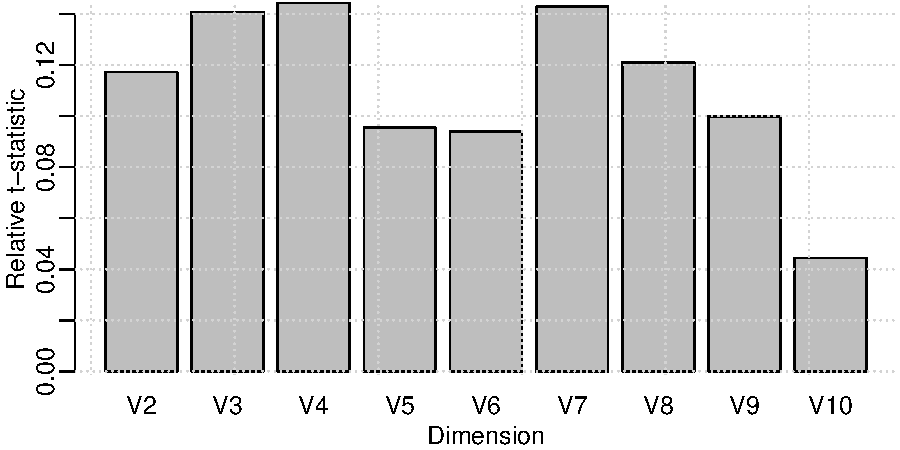
\includegraphics[width=\linewidth]{images/tumor_ttest.pdf}
  \end{minipage}
  \hfill
  \quad
  \begin{minipage}[b]{0.45\linewidth}
    \centering
    \begin{tabular}[b]{c|lll}
      & \textbf{full} & \textbf{$t$-test} & \textbf{seq-fwrd} \\
      \hline
      rand.~acc.   & 96\%   & 93.14\% & 97.1\% \\ 
      $n$-way acc. & 95.7\% & 94.7\%  & 95.1\% \\
      dims         & all    & 2,3,6   & 1,3,6 \\
      $J_1$        & 1.30   & 2.01    & 1.67 \\
      $J_2$        & 6.11   & 4.96    & 5.23 \\
      $J_3$        & 5.11   & 3.96    & 4.23 \\
    \end{tabular}
    \vspace{5mm}
  \end{minipage}
  \hfill
  \vspace{5mm}
  \quad
  \begin{minipage}[t]{1.00\linewidth}
    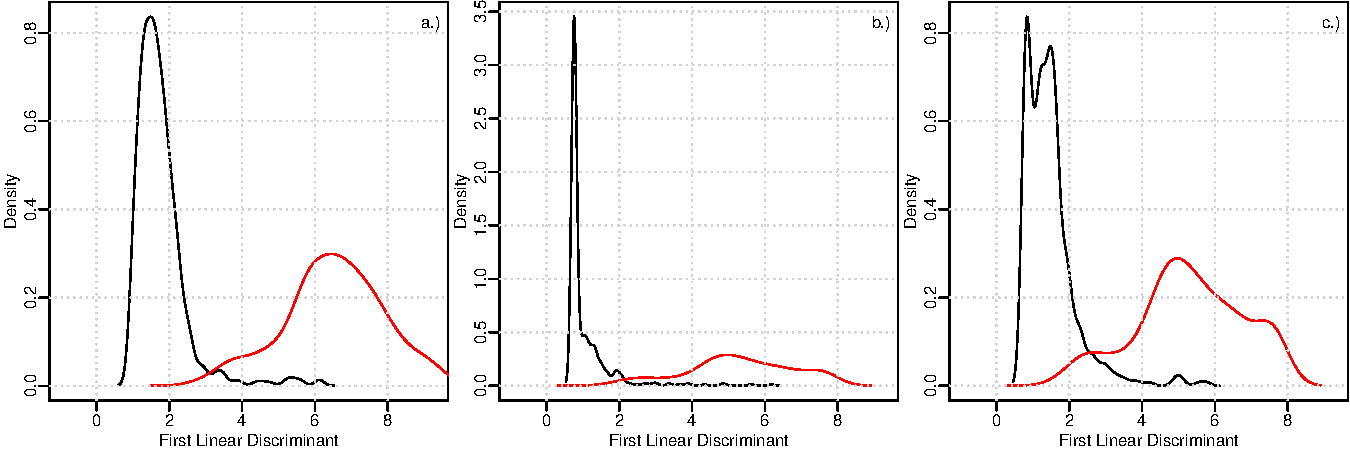
\includegraphics[width=\linewidth]{images/tumor.pdf}
  \end{minipage}
  \caption{The density of the \texttt{tumor} data projected onto the first linear discriminant using: a.) all the dimensions; b.) three best dimensions resulting from the relative-$t$-test (top left barplot); and c.), three best dimensions determined from the sequential-forward algorithm.  The random 75\% training data score, leave-one-out-cross-validation score, best dimension indicies, and $J$-scores are provided in the above right table for the full model, $t$-test-best-dimensions model, and sequential-forward-best-dimensions model.   Note that the sequential-forward-derived dimensions performed slightly better than the $t$-test-derived dimensions, despite having a lower $J_1$ score.}
\end{figure}

\section{mouse data}

\begin{figure}[H]
  %\centering
  \begin{minipage}[b]{0.65\linewidth}
    \hspace{5mm}
    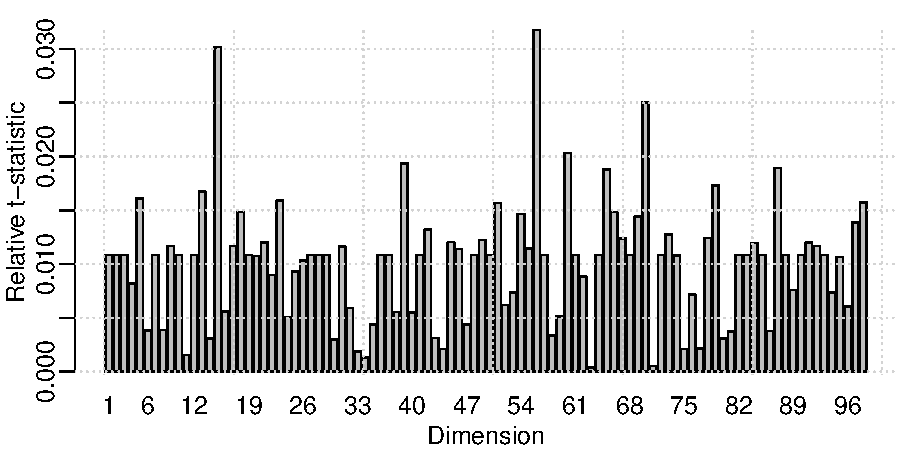
\includegraphics[width=\linewidth]{images/mouse_ttest.pdf}
  \vspace{10mm}
  \end{minipage}
  \hfill
  \quad
  \begin{minipage}[b]{0.45\linewidth}
    \centering
    \begin{tabular}[b]{c|c|c}
      \textbf{dims} & \textbf{accuracy} & \textbf{method} \\
      \hline
      5   & 75\% & t-test \\
      12  & 85\% & seq-fwrd\\
      13  & 80\% & seq-fwrd\\
      14  & 70\% & seq-fwrd\\
      15  & 65\% & seq-fwrd\\
    \end{tabular}
    \vspace{20mm}
  \end{minipage}
  \hfill
  \vspace{10mm}
  \quad
  \begin{minipage}[t]{1.00\linewidth}
    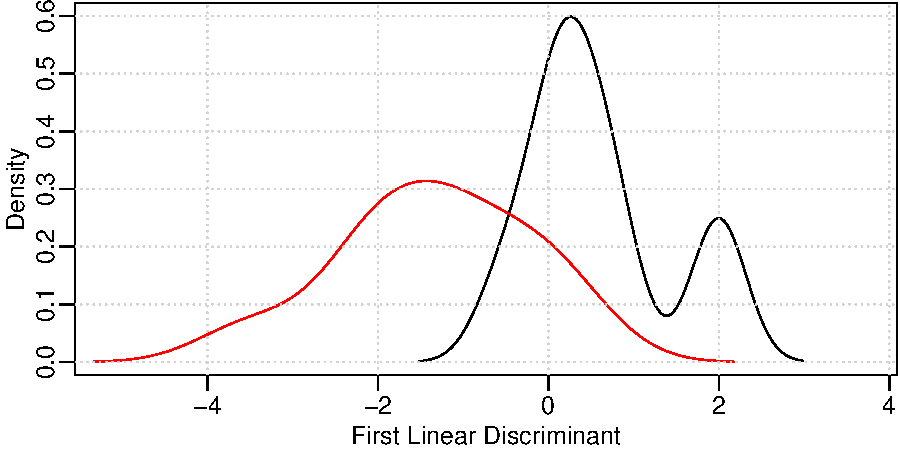
\includegraphics[width=\linewidth]{images/mouse.pdf}
  \end{minipage}
  \caption{The density of the \texttt{mouse} data projected onto the first linear discriminant using the five-best dimensions from the relative-$t$-test (top left barplot).  The table (upper right) gives the performance for the sequential-forward $n$-best dimensions.  Note that as the number of dimensions increases, the $n$-way-cross-validation scores decrease.} 
\end{figure}

\section{fertility dataset}

\begin{figure}[H]
  %\centering
  \begin{minipage}[b]{0.45\linewidth}
    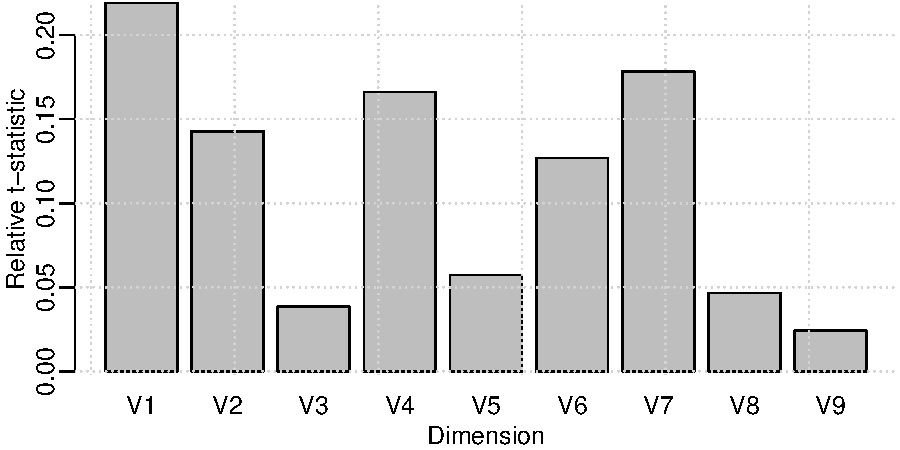
\includegraphics[width=\linewidth]{images/fertility_ttest.pdf}
  \end{minipage}
  \hfill
  \quad
  \begin{minipage}[b]{0.45\linewidth}
    \centering
    \begin{tabular}[b]{c|lll}
      & \textbf{full} & \textbf{$t$-test} & \textbf{seq-fwrd} \\
      \hline
      rand.~acc.   & 92\%                        & 92\%       & 92\% \\ 
      $n$-way acc. & 85\%                        & 86\%       & 86\% \\
      dims         & all                         & 1,2,4,6,7  & 1,2,4,6,7 \\
      $J_1$        & $1.57 \times 10\sups{-2}$   & $2.73 \times 10\sups{-2}$ & $2.73 \times 10\sups{-2}$ \\
      $J_2$        & 1.13  & 1.12       & 1.12 \\
      $J_3$        & 0.132 & 0.117      & 0.117 \\
    \end{tabular}
    \vspace{5mm}
  \end{minipage}
  \hfill
  \vspace{5mm}
  \quad
  \begin{minipage}[t]{1.00\linewidth}
    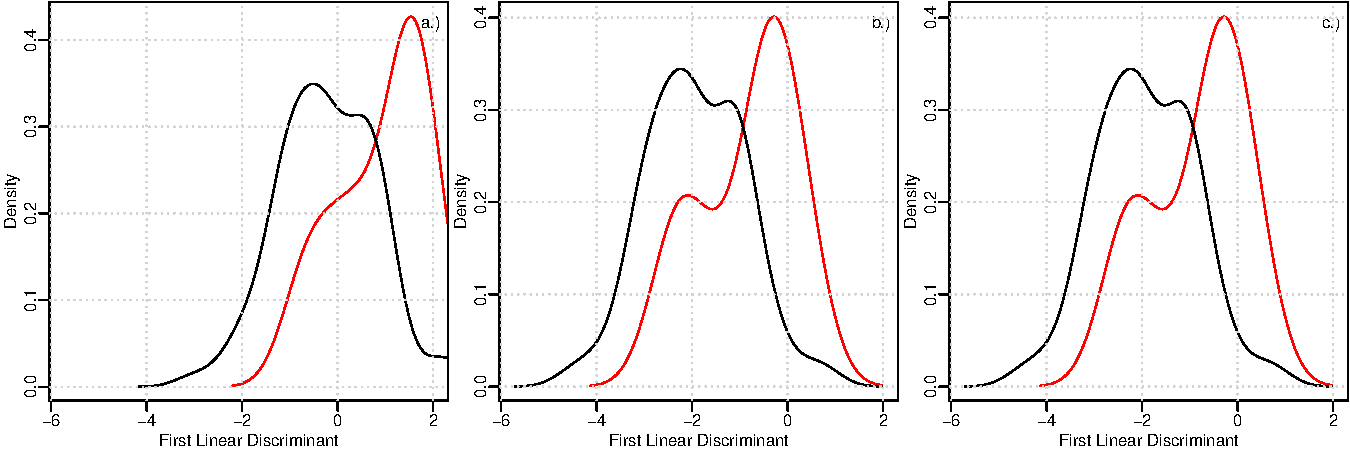
\includegraphics[width=\linewidth]{images/fertility.pdf}
  \end{minipage}
  \caption{The density of the \texttt{fertility} data projected onto the first linear discriminant using: a.) all the dimensions; b.) five best dimensions resulting from the relative-$t$-test (top left barplot); and c.), five best dimensions determined from the sequential-forward algorithm -- indentical to the $t$-test-derived dimensions.  The random 75\% training data score, leave-one-out-cross-validation score, best dimension indicies, and $J$-scores are provided in the above right table for the full model, $t$-test-best-dimensions model, and sequential-forward-best-dimensions model.   Note that reduced-dimensional models performed slightly better than the full-dimensional model.}
\end{figure}

\newpage

\section{source code}

\begin{multicols}{2}

\subsection{functions}

\Rexternal{../src/functs.r}

\subsection{iris data}

\Rexternal{../src/iris.r}

\subsection{fruit data}

\Rexternal{../src/fruit.r}

\subsection{tumor data}

\Rexternal{../src/tumor.r}

\subsection{mouse data}

\Rexternal{../src/mouse.r}

\subsection{fertility data}

\Rexternal{../src/fertility.r}


\end{multicols}

%\begin{figure}[H]
%  \centering
%    \includegraphics[width=\linewidth]{images/.png}
%\end{figure}


\end{document}


